\chapter{Case studies}
\label{chp:case_studies}
% ------------------------------------------------------------------------------

\noindent{\LARGE\textbf{Case study 1}}\\
% ==============================================================================
\section{A mechanistic emulator: fitting the \emph{weir equation}}
% ==============================================================================

% ::::::::::::::::::::::::::::::::::::::::::::::::::::::::::::::::::::::::::::::
%  * present it as a didactic example
%  * use it to compare GP (prior knowledge) with e.g. deep neural networks: how many points can we have?
%  * mention grid convergence study (results go in the appendix)
%  * mention problem with FullSWOF boundary conditions
%  * define well results and methodology
%  * such an emulator can be improved -> modified to compute slope in order to have a given mu value
%  * state all of the goals of the CS: learn weir eq. from simulation, apply curve fitting, get a feeling for simulation accuracy
% ::::::::::::::::::::::::::::::::::::::::::::::::::::::::::::::::::::::::::::::

As a first case study to apply the acquired knowledge, it was decided to build an utterly mechanistic emulator.
The main goal of this case study is to try to fit the \emph{weir equation} to simulated data instead of to experimental data.
Here we basically rediscover the way science has always been done, by observing, measuring and trying to find mathematical relationships, with the biggest difference being the fact that the experimental set-up is completely computer built.\\

The \emph{weir equation} is a partially theoretical equation that computes the discharge $Q$ over a weir as a function of the water depth above the weir itself ($h_w$).
The equation can be derived from the Bernoulli equation under certain assumptions \autocite{bos_discharge_1989} and can be found under many different forms.
The form used here is the one proposed by \emph{Francis} \autocite{walcott_weir_1907}.

\begin{equation}\label{eq:weir_eq}
  Q = C \cdot L \cdot h_w^{3/2}
\end{equation}

\noindent Where the empirical coefficients $C$ corrects for the assumption of absence of viscous effects and uniform velocity distribution. $L$ is the length of the weir (perpendicular to the channel) and $h_w$ is the water height above the weir.

In addition to the parametric model (weir equation) two non-parametric local techniques, namely \emph{linear interpolation} and \emph{cubic spline interpolation}, were used to intrapolate between the data points.\\


% ------------------------------------------------------------------------------
\subsection{Brief experiment description}
% ------------------------------------------------------------------------------

\seb{explain the experiment very generally. Put the section title or leave it with no section title with the upper part?}
 
 For this experiment simulations were run in a flat rectangular channel.
A weir with a trapezoidal cross section is located at the channel half-length.
As initial condition the upstream side of the weir was filled with water up to the weir crest.
At the domain top boundary a constant inflow discharge was set, while at the bottom boundary water could freely outflow.
As the simulation runs, the inflow water flows down the channel, overflows the weir and leaves the domain through the lower boundary.
After some time the simulation reaches the \emph{steady-state conditions}: inflow, discharge over the weir and outflow have the same magnitude and the water height above the weir, measured \SI{1.2}{\meter} before the weir, has stabilized.
At this point the value $h_w$ was extracted and was coupled with the discharge value $Q$ generating it.
This pair $(Q, h_w)$ constitute a \emph{predictor-response} set of the dataset to which the weir equation was fitted.
This procedure was applied to all of the experiments run, where only the inflow value $Q$ was varied from one experiment to the other.
\num{25} experiments were conducted with $Q$ linearly spaced in the range \SIrange{0.1}{10}{\cubic\meter\per\second}.\\

In order to ensure the convergence of the simulator solution, and therefore the quality of the experimental results, a \emph{grid convergence study} was performed prior to the experiment.
For this, the simulation with the highest discharge was repeated with successive grid refinements
The value of the variable of interest, water height, was then compared between the different simulations to find at which grid resolution the solution has stabilized.


% ------------------------------------------------------------------------------
\subsection{Material and methods}
% ------------------------------------------------------------------------------

\subsubsection{Generating the topography}

The topography used for running the simulations was generated in \textit{Octave} and represents a flat channel of \SI{40}{\meter} length with a weir placed at its midpoint, at \SI{20}{\meter} distance from the top boundary.
The channel cross section is a rectangle of \SI{4}{\meter} width and the weir has a trapezoidal shape.
Fig.~\ref{fig:weir_scheme} shows the geometry of the channel.
The weir has a crest width of \SI{2}{\meter} and therefore belongs to the \emph{broad-crested} class. The $C$ coefficient for broad-crested weirs with vertical walls and \SI{2}{\meter} crest width varies between \num{1.36} and \num{1.53}, depending on the water height $h_w$ \autocite{brown_urban_2009}.
We therefore expect a value close to this. A 3D overview of the channel can be found in the appendix \ref{app:channel_topography} \seb{add a 3D plot of the channel?}.

\begin{figure}[h]
  \centering
  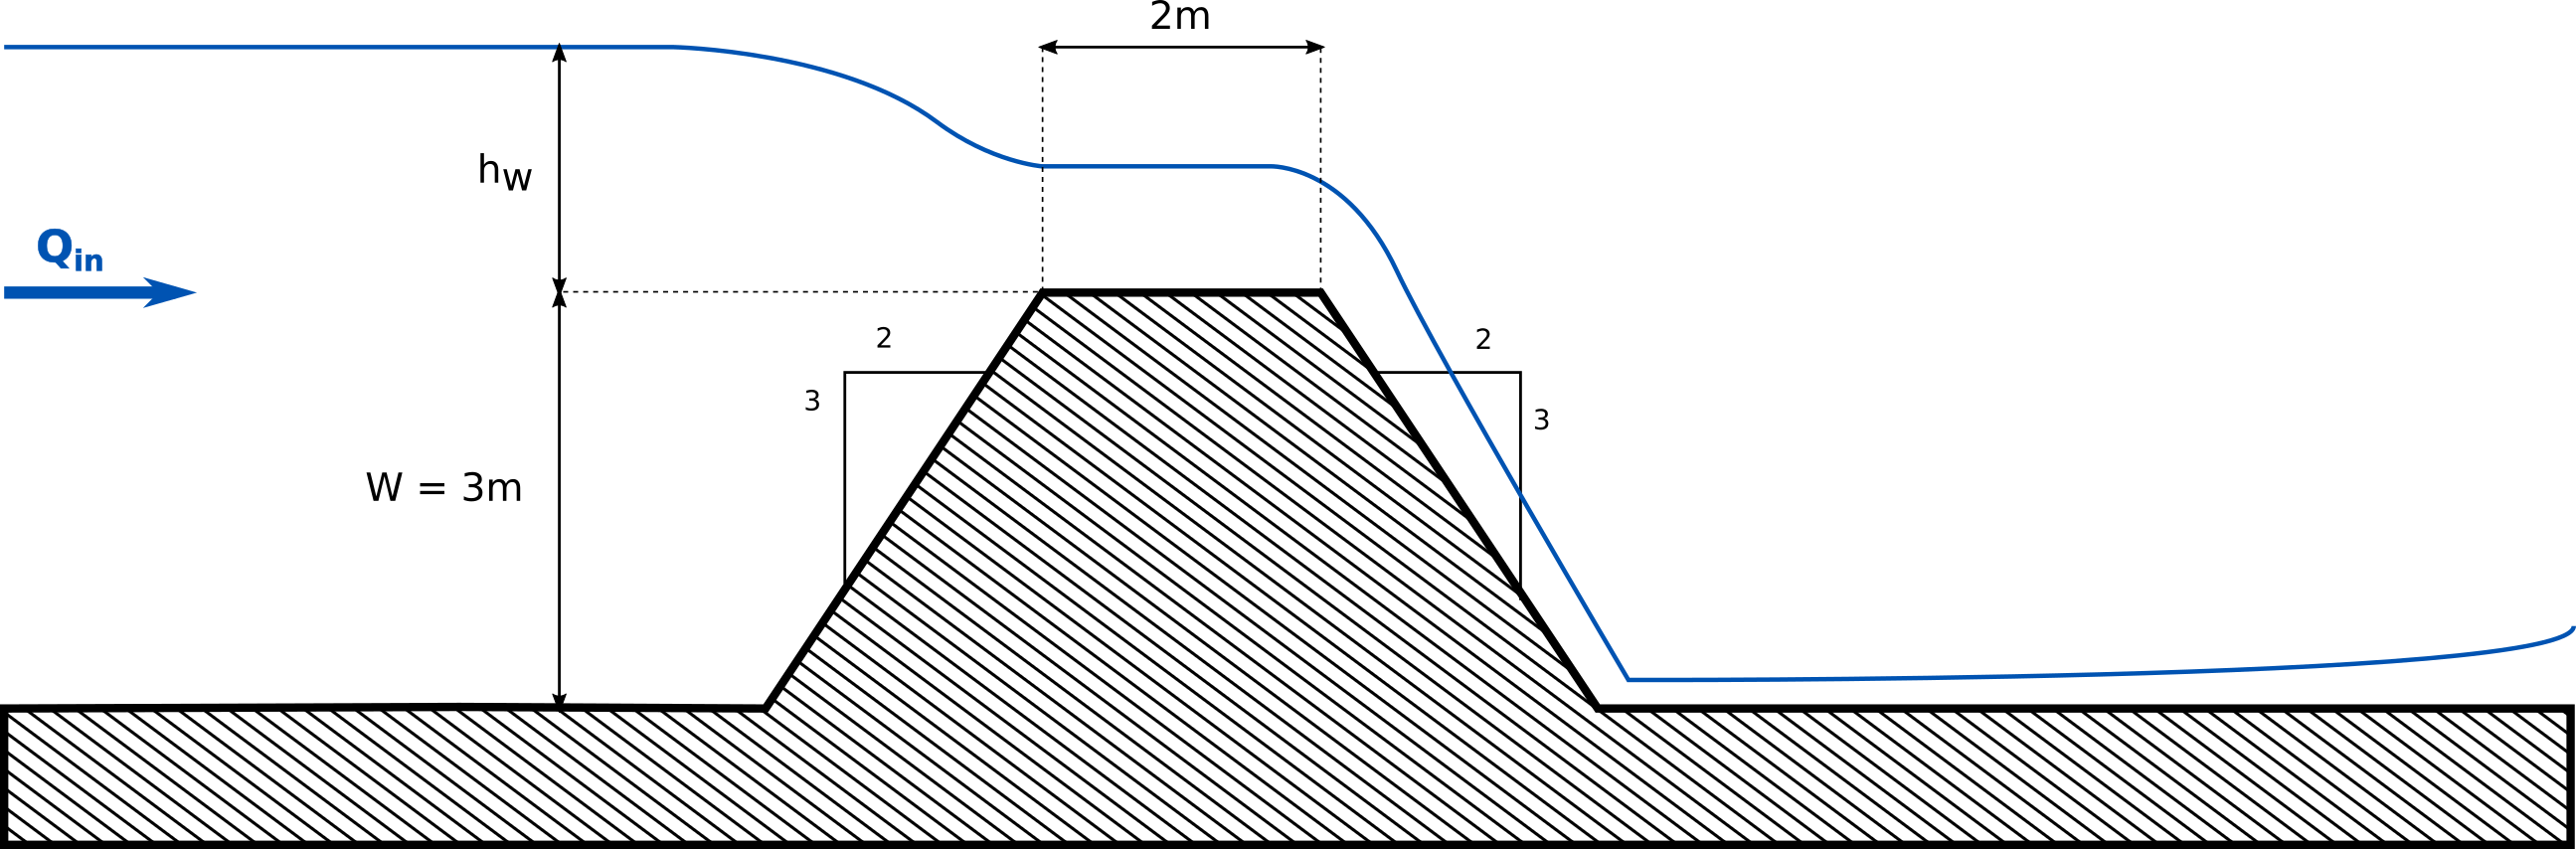
\includegraphics[width=0.8\textwidth]{Figures/weir_scheme.png}
  \caption{fig:Weir bla bla}
  \label{fig:weir_scheme}
\end{figure}


\subsubsection{Performing the grid convergence study}

Accuracy of simulation results, as well as simulation runtime, are dependent on the mesh resolution chosen.
In order to find an appropriate mesh resolution, a \emph{mesh study} has to be run before the actual experiment is performed.
Increasing grid refinements are tested for the problem which is to solve and a convergence criterion is established.
If the Grid Convergence Index (GCI) is used, then a GCI lower than \SI{5}{\percent} for the last refinement is usually taken as a criterion \autocite{ali_grid_2009}.\\

For the mesh study \num{7} simulations were run by varying only the grid resolution.
Squared cells were used and the inflow discharge was set to the highest discharge value of the experiment, corresponding to \SI{10}{\cubic\meter\per\second}.
This discharge is the one generating the highest flow velocities.
If convergence under these conditions is reached, then convergence for lower discharges is also assured.

\begin{table}[h]
  \centering
  \caption{Summary of simulations runtime, grid resolution and other related parameters for the mesh convergence study.}
  \label{tab:mesh_study}
  \begin{tabular}{crrcccccr}
    \toprule
%    \rowfont{\bfseries}
    \multirow{2}{*}{\#} & \multicolumn{1}{c}{Nx} & \multicolumn{1}{c}{Ny} & \multicolumn{1}{c}{Lx} & \multicolumn{1}{c}{Ly} & \multicolumn{1}{c}{dx} & \multicolumn{1}{c}{dy} & \multicolumn{1}{c}{Q} & \multicolumn{1}{c}{runtime} \\
       & \multicolumn{1}{c}{$[\mbox{--}]$} & \multicolumn{1}{c}{$[\mbox{--}]$} & \multicolumn{1}{c}{$[\si{\meter}]$} & \multicolumn{1}{c}{$[\si{\m}]$} & \multicolumn{1}{c}{$[\si{\m}]$} & \multicolumn{1}{c}{$[\si{\m}]$} & \multicolumn{1}{c}{$[\si{\cubic\m\per\s}]$} & \multicolumn{1}{c}{$[\si{\minute}]$} \\
    \midrule
    1  & 2             & 20            & 4               & 40          & 2.00        & 2.00        & 10                      & 0.00 \\
    2  & 4             & 40            & 4               & 40          & 1.00        & 1.00        & 10                      & 0.07 \\
    3  & 8             & 80            & 4               & 40          & 0.50        & 0.50        & 10                      & 0.60 \\
    4  & 20            & 200           & 4               & 40          & 0.20        & 0.20        & 10                      & 9.00 \\
    5  & 40            & 400           & 4               & 40          & 0.10        & 0.10        & 10                      & 69.60 \\
    6  & 80            & 800           & 4               & 40          & 0.05        & 0.05        & 10                      & 537.72 \\
    7  & 100           & 1'000         & 4               & 40          & 0.04        & 0.04        & 10                      & 1'048.40 \\
    \bottomrule
  \end{tabular}
\end{table}


% ------------------------------------------------------------------------------
\subsection{Results and discussion}
% ------------------------------------------------------------------------------

Present and discuss briefly the results of this toy emulator.\\


% ------------------------------------------------------------------------------
%An \textit{early flood warning tool} in an essential component of an \textit{early flood warning system}.
%An early flood warning system has to be understood as an integrated system of tools and plans to detect and respond to flood emergencies \autocite{icimod_early_2018}.
%This can be managed by the community themselves and if designed, implemented and operated correctly can make the difference between tragedy and survival.

%Such systems have already been installed in various endangered regions in the world.
%After the major flooding of July 2014, the city of Altstätten in the canton of St. Gallen made the decision to install one.
%The system installed uses cameras, sensors and level meters to gather data and information about the current situation \autocite{st._galler_tageblatt_altstatten_2017}.
%When the value of certain parameters exceed the given threshold, a dangerous situation is recognized and the alarm signal is sent.

%Three years after the installation of the system an alarm rings in the middle of the night.
%Firemen go immediately into action in order to install temporary measures to fight against the water.
%A couple of hours later the torrent overflows at several points and the city gets flooded.
%Damages are less severe than last time, especially thanks to the temporary measures installed, but possibly they could have been reduced even more.

%Crucial in order to limit the damages is the intervention time before the actual flooding occurs.
%The earlier the dangerous situation can be detected the more time is available to the population and authorities to get ready and set up different types of temporary mitigation measures.
%Systems based on sensors monitoring the evolution of the current situation in the upper part of the catchment are quite reliable but do not allow for long anticipation time.

%Numerical simulations can be run with meteorological forecast data and approximate soil saturation conditions in order to obtain early predictions of the event outcome.
%However, the big advantage of predicting with that much anticipation is partially lost due to the duration of such simulations.
%Accurate meteorological forecasts are available only few hours before the event.
%If the model require several hours to run, which is often the case to obtain accurate predictions for catchments of this extent, then the advantage of being able to run it in advance is canceled.

%A possible solution to this problem is the development of an \emph{early flood warning tool} based on an \emph{ad hoc surrogate model} exploiting the catchment specific behavior.
%This early flood warning tool should be able to recognize if a rain event will generate a channel discharge leading to flooding and if yes within how much time.
%For this scope two different emulators are used.
%The first emulator classifies a rain event based on the forecasted \emph{average rain intensity} and \emph{current soil saturation} into two groups: rain events generating discharge exceeding a chosen threshold ($Q_!$) and rain events not generating discharge exceeding the threshold.
%For events exceeding the threshold a second emulator is developed.
%This predicts the time the rain event will need to produce the threshold discharge $Q_!$ at the outlet of the catchment.
% ------------------------------------------------------------------------------


\newpage

\noindent{\LARGE\textbf{Case study 2}}
%===============================================================================
\section{An hydrological emulator: estimating the \textit{time-to-threshold}}
%===============================================================================

With this case study it was decided to address a complex hydrological problem by means of emulation.
The problem we want to solve is estimating the time needed for a channel conveying water from a catchment to reach a certain threshold discharge ($Q_!$) at its outlet as a function of rain intensity and initial soil saturation.

For the experiment a synthetic catchment topography was used, which at first glance can make the case study look very abstract.
In reality the emulator is just exploiting the catchment specific behavior, which is of course different from one catchment to another, but the methodology applied here could be applied to whatever catchment.
The emulator developed here, with the appropriate adjustments, could be exploited as an \emph{early flood warning tool}.

As for the previous example, the simulations were run with the open source software \textit{FullSWOF\_2D-v.1.07.00} \autocite{delestre_fullswof:_2014} \seb{put the citation every time that it is mentioned?}, while the input files necessary for the simulations were prepared with \textit{GNU Octave 4.2.1} \autocite{octave_community_gnu_2018} \seb{how to cite this?} with the aid of the package \textit{fswof2d}.


% ------------------------------------------------------------------------------
\subsection{Material and methods}
% ------------------------------------------------------------------------------

\subsubsection{The synthetic topography}

The topography used represents a catchment of size $\SI{2}{\kilo\meter} \times \SI{2}{\kilo\meter}$ and it is visible in Fig~\ref{fig:topography}.
It is composed of a sloping plane with three Gaussian bumps on the top.
The Gaussian bumps have different heights and widths and generate a \emph{Y-shaped channel} which extends from the upper and left boundary down to the lower boundary.
A paraboloid was added to the plane to promote the accumulation of water in the channel.
This has a single outlet located close to the center of the domain's bottom boundary.

The synthetic topography produced, in contrast to a real one, has the advantage of having a much smoother surface, which allows using a coarser grid resolution without losing topographical features.
The coarser the grid the fewer the nodes where the finite volume (FV) equations have to be solved, which reduces the simulation runtime \seb{how does it decrease? linearly? quadratically?}. 
Another advantage of having a smooth topography, not presenting discontinuities, is that the solutions converge easily, and no grid refinement is necessary.
The grid used is composed of $\num{100} \times \num{100}$ cells, giving a resolution of $\SI{20}{\meter} \times \SI{20}{\meter}.$

\begin{figure}[h]
  \centering
  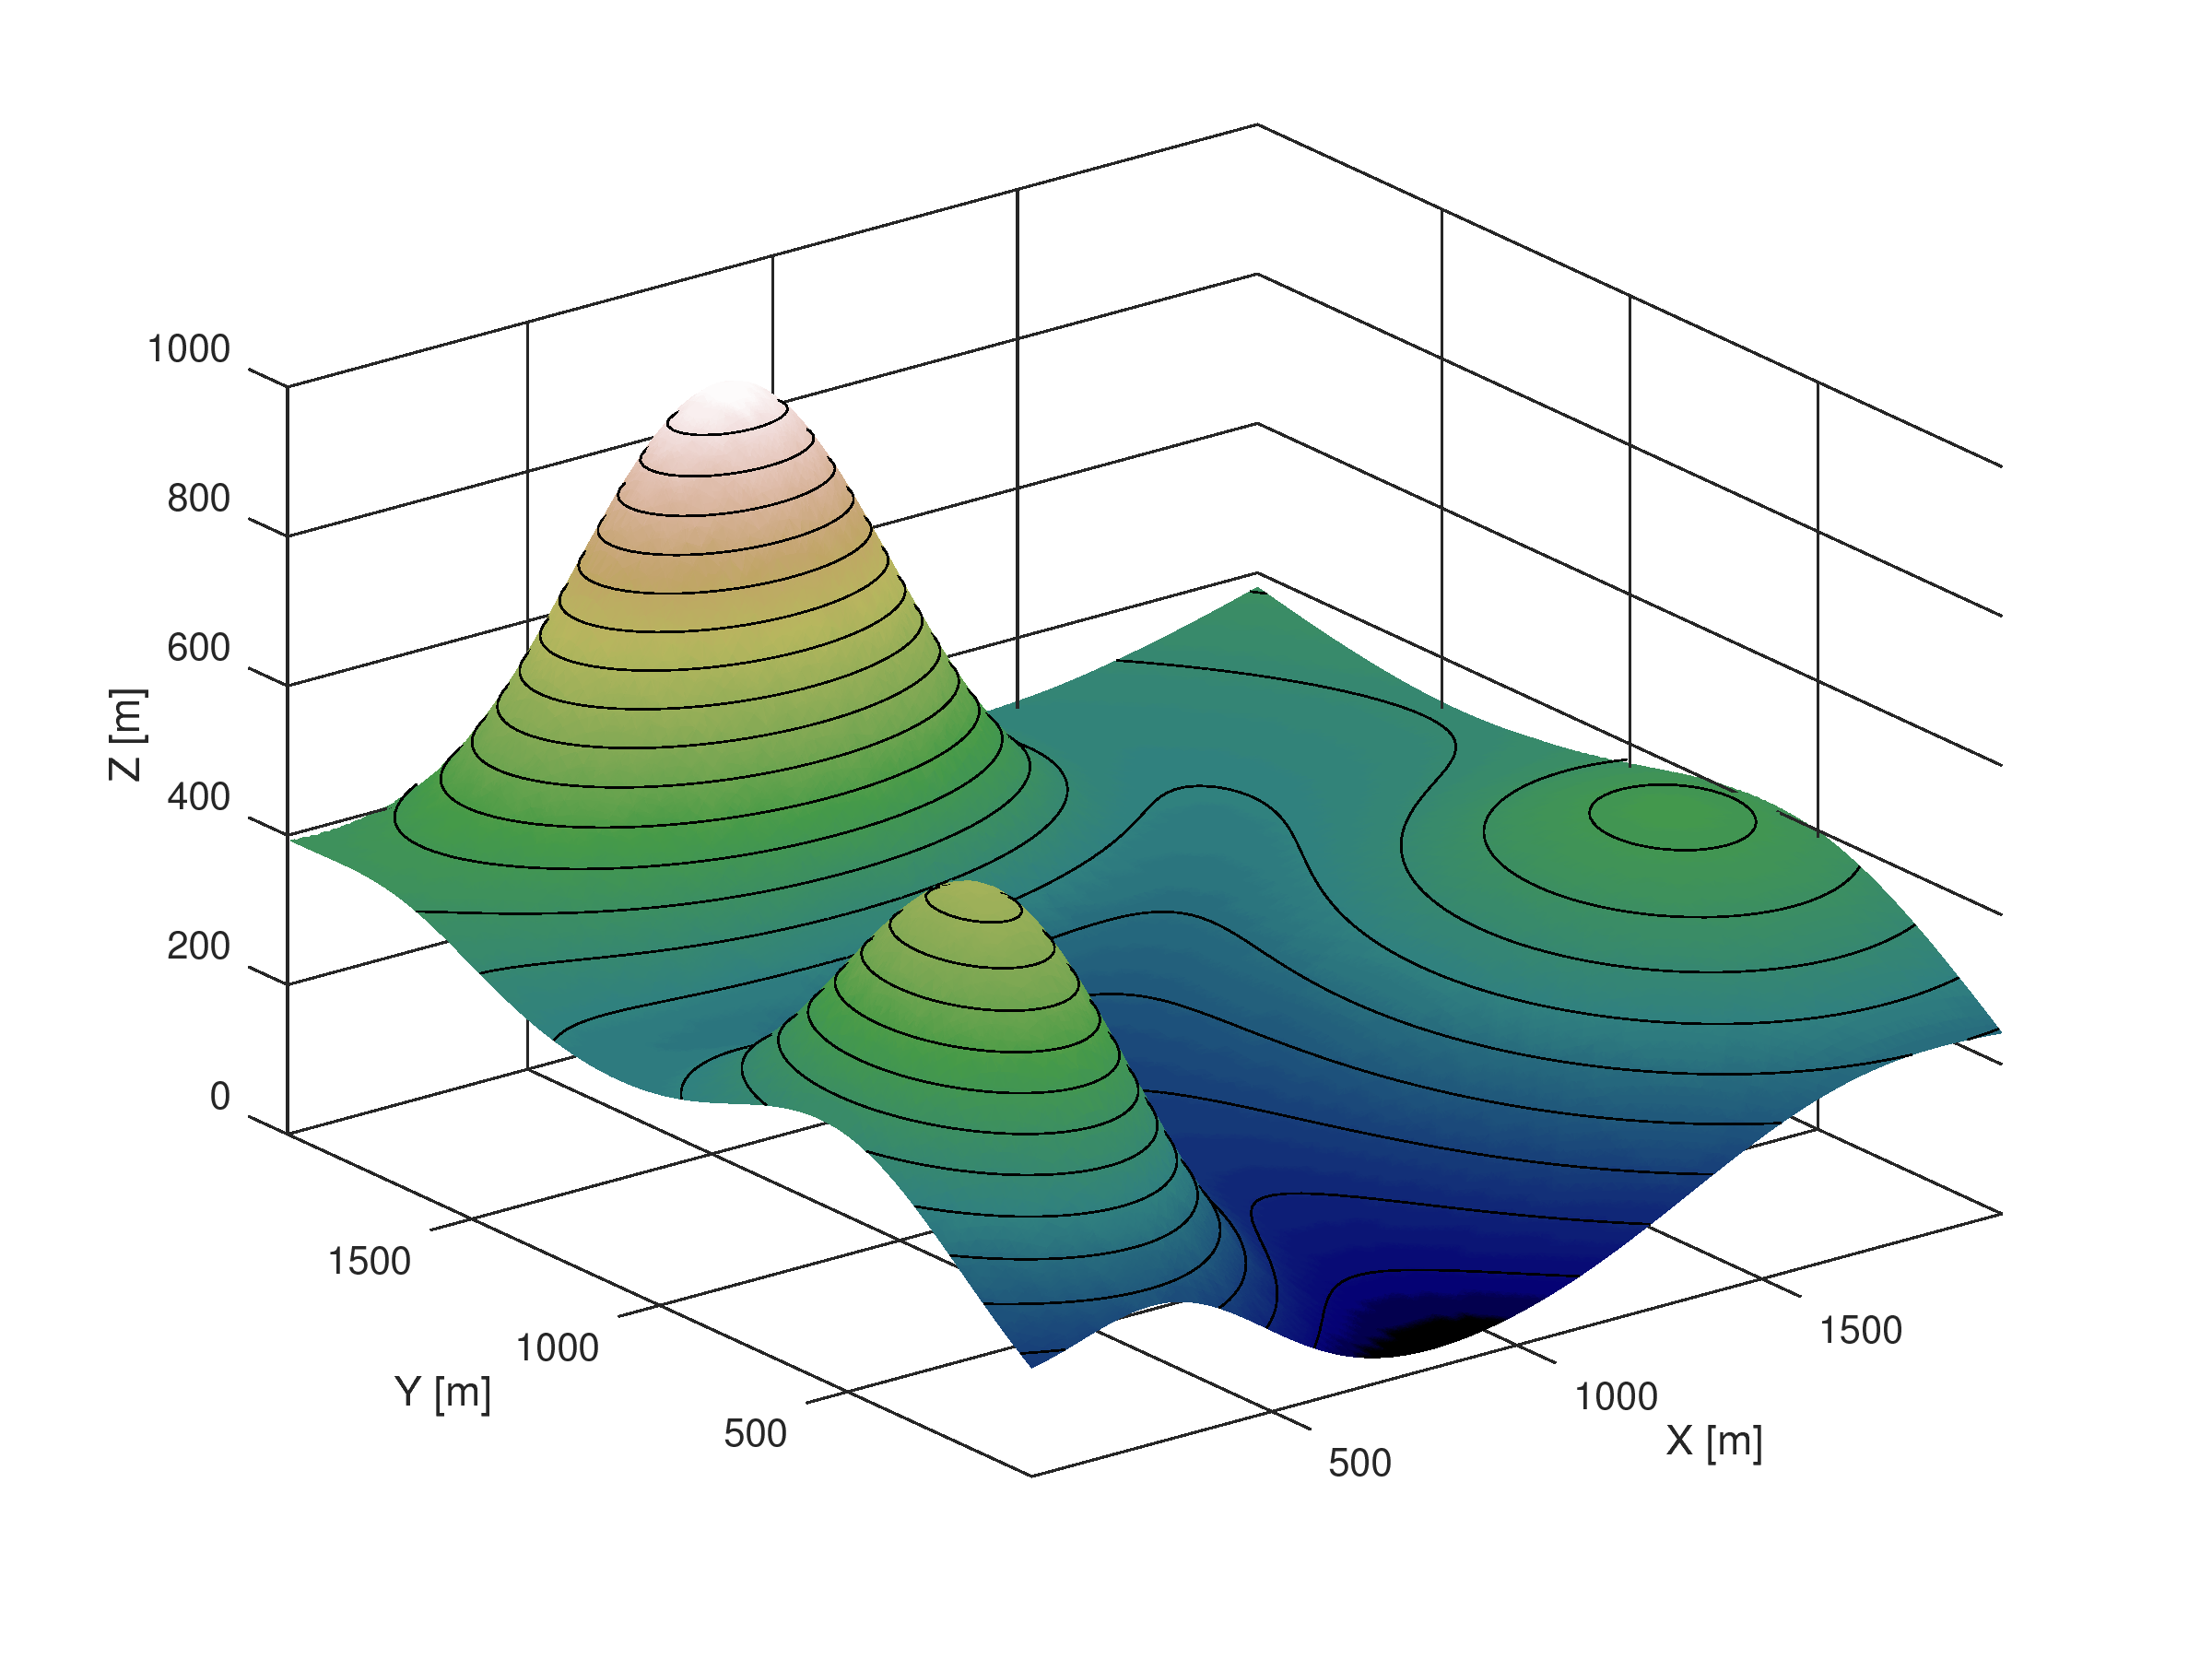
\includegraphics[width=0.7\textwidth]{Figures/topography.png}
  \caption{Synthetic topography composed of three Gaussian bumps on a sloping plane.}
  \label{fig:topography}
\end{figure}


\subsubsection{Setting-up the simulations}

The dataset required for building the emulator was generated by running \num{50} simulations with different combinations of the variables \emph{rain intensity} ($I$) and \emph{initial soil saturation} ($\theta_i$).
The initial soil saturation, being a spatially distributed variable, was kept uniform over the whole domain.
The rain intensity was kept constant and was uniformly applied over the domain, also since \textit{FullSWOF\_2D}, at this stage of development, only allows for uniformly distributed rain events \autocite{laguerre_documentation_2016}.

\num{5} different initial saturations in the $[\numrange{0}{1}]$ interval and \num{10} rain intensities in the \SIrange{10}{35}{\milli\metre\per\hour} interval were taken and all their possible combinations were used as inputs for the simulations.
The rain duration was set to \SI{6}{\hour}, while a simulation duration of \SI{9}{\hour} was chosen in order to be able to observe the hydrograph recession. A time resolution of \SI{60}{\second} was used, which means that intermediate simulation results were written to the \emph{outputs} file every \SI{60}{\second}.

Some parameters, namely those specific for the catchment in questions, were kept constant over all of the simulations.
These are summarized in Tab.~\ref{tab:simulations_parameters}.
The parameters marked with * are those \emph{spatially distributed}, meaning that a different value could be set for every cell.
For simplicity, a spatially uniform catchment was used, therefore the values from the table are valid for the whole domain.
Three \textit{wall boundary conditions} were set, for the upper and the two lateral boundaries.
For the bottom boundary a \textit{Neumann boundary condition} was selected, allowing water to freely outflow through that boundary and making sure that all of the water is lost from here.

\begin{table}[h]
  \centering
  \caption{Parameters and setting fixed for all simulations.}
  \label{tab:simulations_parameters}
  \begin{threeparttable}
    \begin{tabular}{lrl}
      \toprule
      \textbf{Parameter} & \textbf{Value} & \textbf{Units} \\
      \midrule
      Domain x-length                          &    $2'000$           & \si{\meter}   \\
      Domain y-length                          &    $2'000$           & \si{\meter}   \\
      Number of cells x                        &    $100$             & --   \\
      Number of cells y                        &    $100$             & --   \\
      Friction coefficient\tnote{*}            &    $0.03$            & \si{s.m^{-1/3}}\\
      Crust thickness\tnote{*}                 &    $1$               & \si{\meter}\\
      Crust hydraulic conductivity\tnote{*}    &    $2\cdot 10^{-6}$  & \si{\meter\per\second}\\
      Soil hydraulic conductivity\tnote{*}     &    $2\cdot 10^{-6}$  & \si{\meter\per\second}\\
      Soil suction head\tnote{*}               &    $0.09$      & \si{\meter}\\
      Soil maximum infiltration rate\tnote{*}  &    $19.8$      & \si{\milli\meter\per\hour}\\
      \bottomrule
    \end{tabular}
    \begin{tablenotes}
      \item[*] Parameters spatially distributed.
    \end{tablenotes}
  \end{threeparttable}
\end{table}


\subsubsection{Extracting the datasets}

%This data constitute the \emph{training} dataset for the emulator.
%A \emph{test} dataset and a \emph{validation} dataset were also generated and can be found in the Appendix~\ref{Appendix}. \seb{verify if they are really added}



The datasets used to build the emulator was extracted from the simulation outputs.
The extraction was done in two steps.
In the first step the outflow hydrographs were extracted from the output data. 
This was done by summing up the cell discharge along the whole domain bottom boundary for every saved time-step (one value every \SI{60}{\second}).
Result of this operation is a discharge values time series of \num{540} elements.
The same procedure was repeated with every one of the \num{50} experiments.

Fig.~\ref{fig:hydrographs3d} shows the extracted hydrographs.
Here many interesting features can be observed.
First of all it can be seen that experiments run with the two lowest rain intensities and low initial soil saturation generated no discharge.
In the second place, simulations run with $\theta_i = \num{1}$ always reached their peak discharge, and this happens quite quickly.
Some of these show a second smaller increase after the first quick rising limb.
This gets higher the higher the rain intensity.
Some simulations show two "increase bumps" after the first rising limb.
This effect is due to the topography.
The topography used presents zones with very steep slopes and others with very flat ones.
This causes that water droplets at the same distance from the outlet to reach it with different travel times.
When the water from the inclines has reached the outlet, that coming from flat areas is still traveling downstream.
After a given lapse of time this water reaches the outlet as well, giving rise to the bumps visible in the hydrographs.\\

\begin{figure}[h]
  \centering
  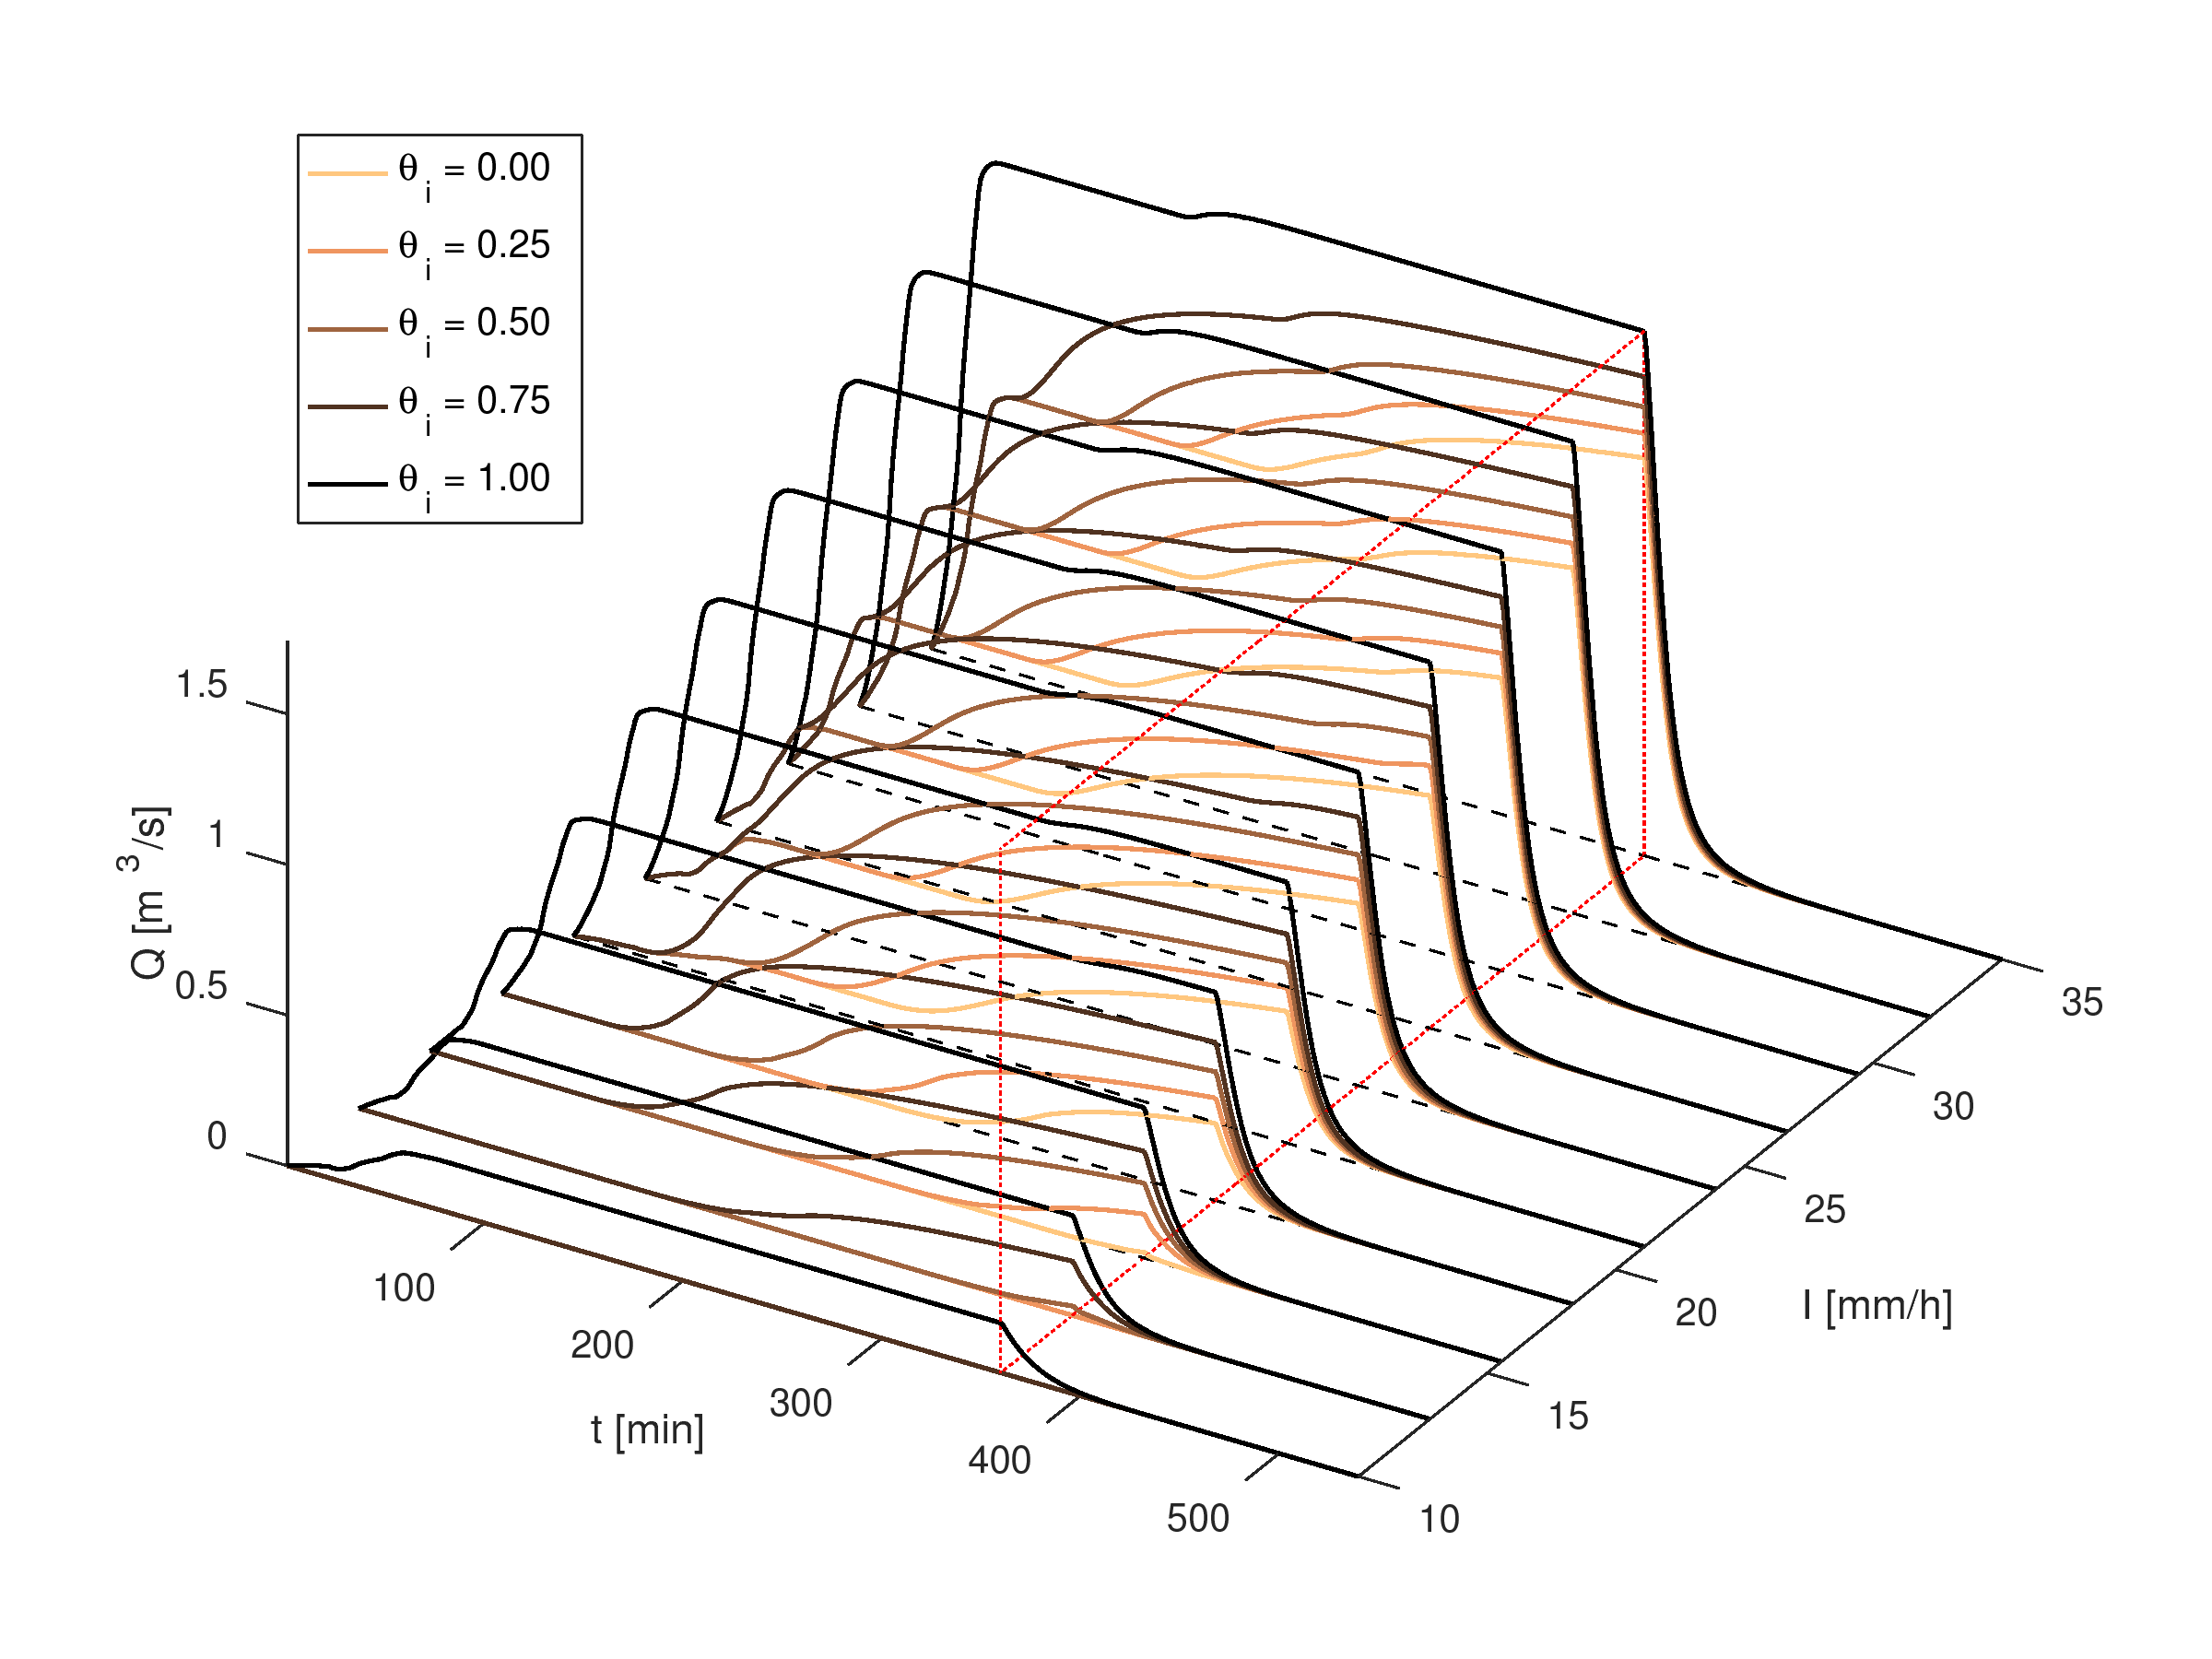
\includegraphics[width=0.75\textwidth]{Figures/hydrographs3d.png}
  \caption{Response hydrographs for the \num{50} simulations at the catchment outlet. The red frame shows the end of the rain event. Depth-dimension shows the \emph{rain intensity} variable, while the \emph{initial saturation} variable is rendered by the colormap.}
  \label{fig:hydrographs3d}
\end{figure}

To build the \emph{time-to-threshold emulator}, the emulator giving the arc of time $t_!$ passed from the beginning of the rain event to the exceeding of the threshold discharge $Q_!$, a threshold discharge has to be established.
For a real case study a characteristic discharge value would be set.
This could be the discharge at which a bridge or the embankments downstream of the considered domain are overflown.
Here this value can be chosen with greater freedom, and the effects of choosing different values can be studied.

By looking at the hydrographs of Fig~\ref{fig:hydrographs3d} it can be observed that $t_!$ is a difficult quantity to predict.
In fact, depending on the $Q_!$ set, there is a variable number of experiments not reaching the threshold, of experiments reaching it very quickly, or of experiment with similar conditions but very different $t_!$.
Especially this last point can be better understood by comparing Fig~\ref{fig:hydrograph}.
The quantity $t_!$ shows discontinuities.
Within the region defined by the $Q_!$ and the $Q'_!$ lines the hydrograph presents a plateau.
Here, a minimal variation of the threshold set can make the time-to-threshold fall towards $t_!$ or $t'_!$, hence causing a big jump in the value.

\begin{figure}[h]
  \centering
  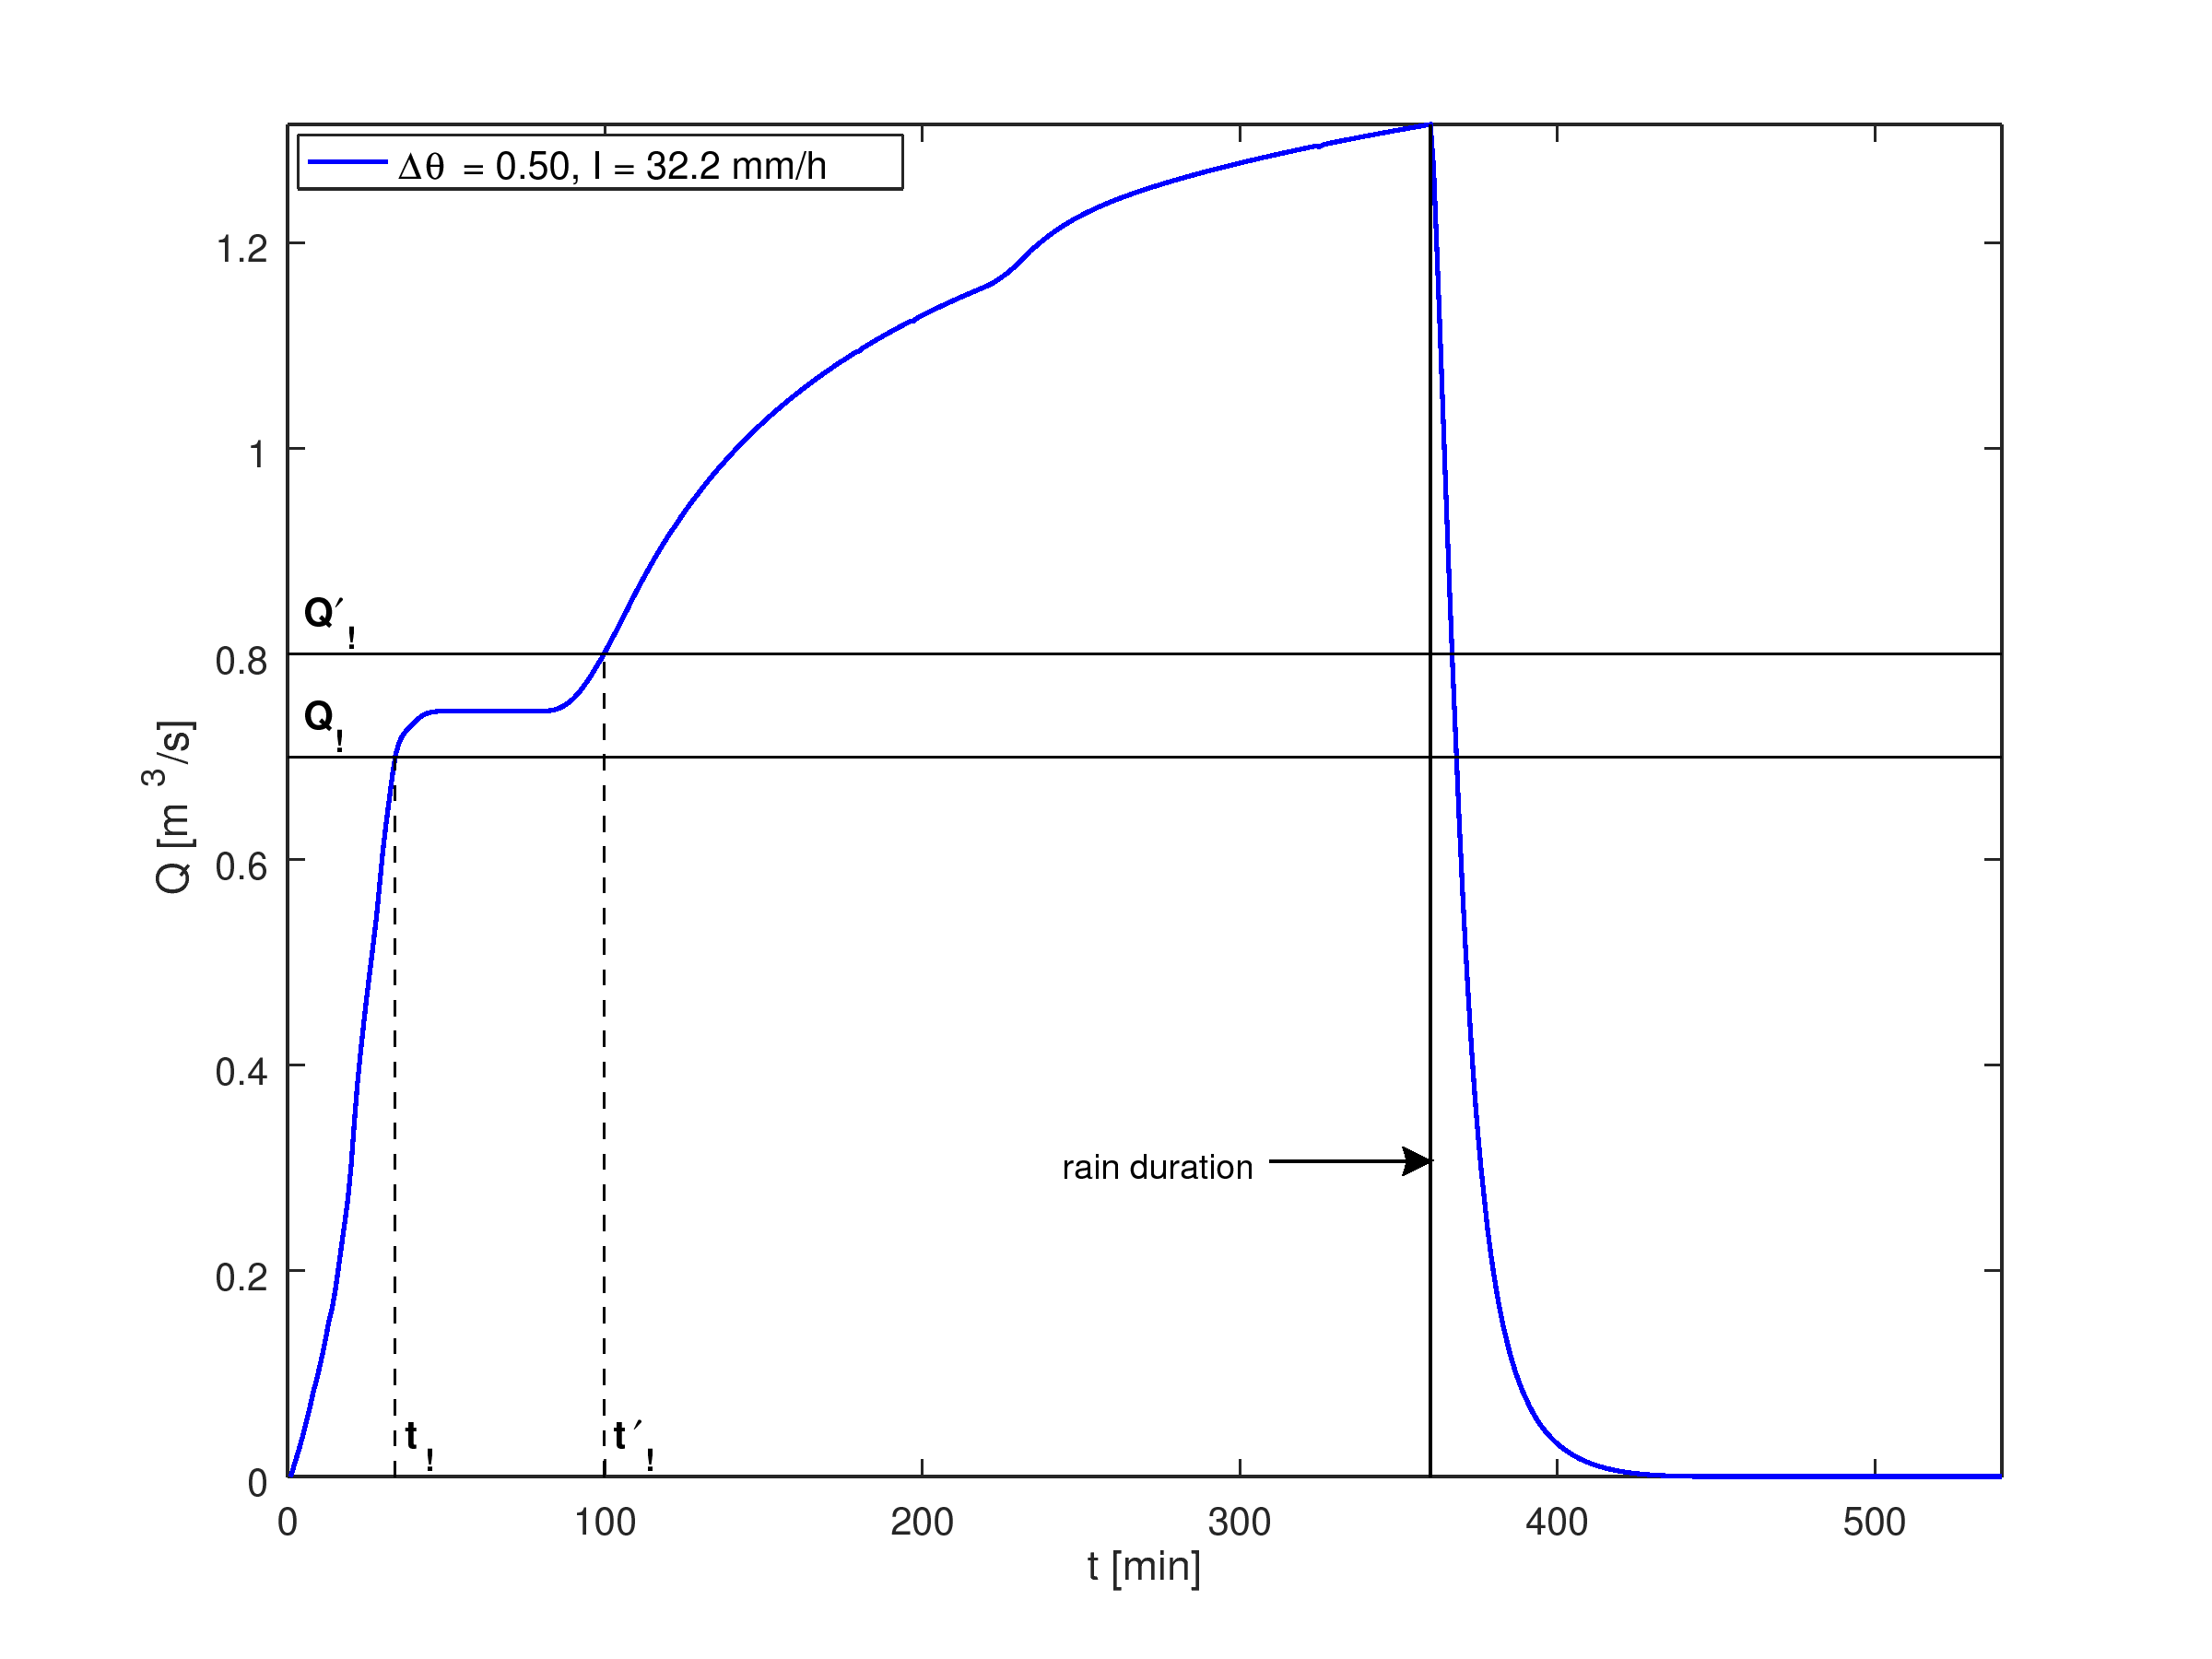
\includegraphics[width=0.7\textwidth]{Figures/hydrograph.png}
  \caption{Response hydrograph for $\theta_i = \num{0.5}$ and $I = \SI{32.2}{\milli\meter\per\hour}$. The discontinuity in the quantity $t_!$ is visible between the $Q_!$ and the $Q'_!$ lines, where the discharge presents a plateau.}
  \label{fig:hydrograph}
\end{figure}

$Q_!$ was set to \SI{10}{\percent} \seb{why this value? should I give any explanation?} of the $Q_{max}$ value recorded, corresponding to \SI{0.17}{\cubic\meter\per\second}.
The time at which this value is exceeded for the first time was extracted from every hydrograph and forms the dataset for the \emph{regression emulator}.
Another dataset for the \emph{classification emulator} was created by assigning the value \num{-1} to rain events not reaching the threshold and \num{1} to all of the others.


\subsubsection{Building-up the classification emulator}


\subsubsection{Building-up the regression emulator}


% ------------------------------------------------------------------------------
\subsection{Results and discussion}
% ------------------------------------------------------------------------------

\begin{itemize}
\itemsep0em
  \item emulator should never underestimate danger (what type of error is this? we want to avoid it absolutely)
  \item try to perform GP interpolation. If it does not work, explain why polynomial interpolation (no time)
  \item use emulator with uncertainty in the $I$ and $\theta_i$. Perform uncertainty quantification
\end{itemize}


\subsubsection{Classification emulator}

Results for the classification emulator
\begin{itemize}
  \item show classification with 3 different $Q_!$
  \item perform testing 
\end{itemize}

\begin{figure}[htpb]
  \centering
  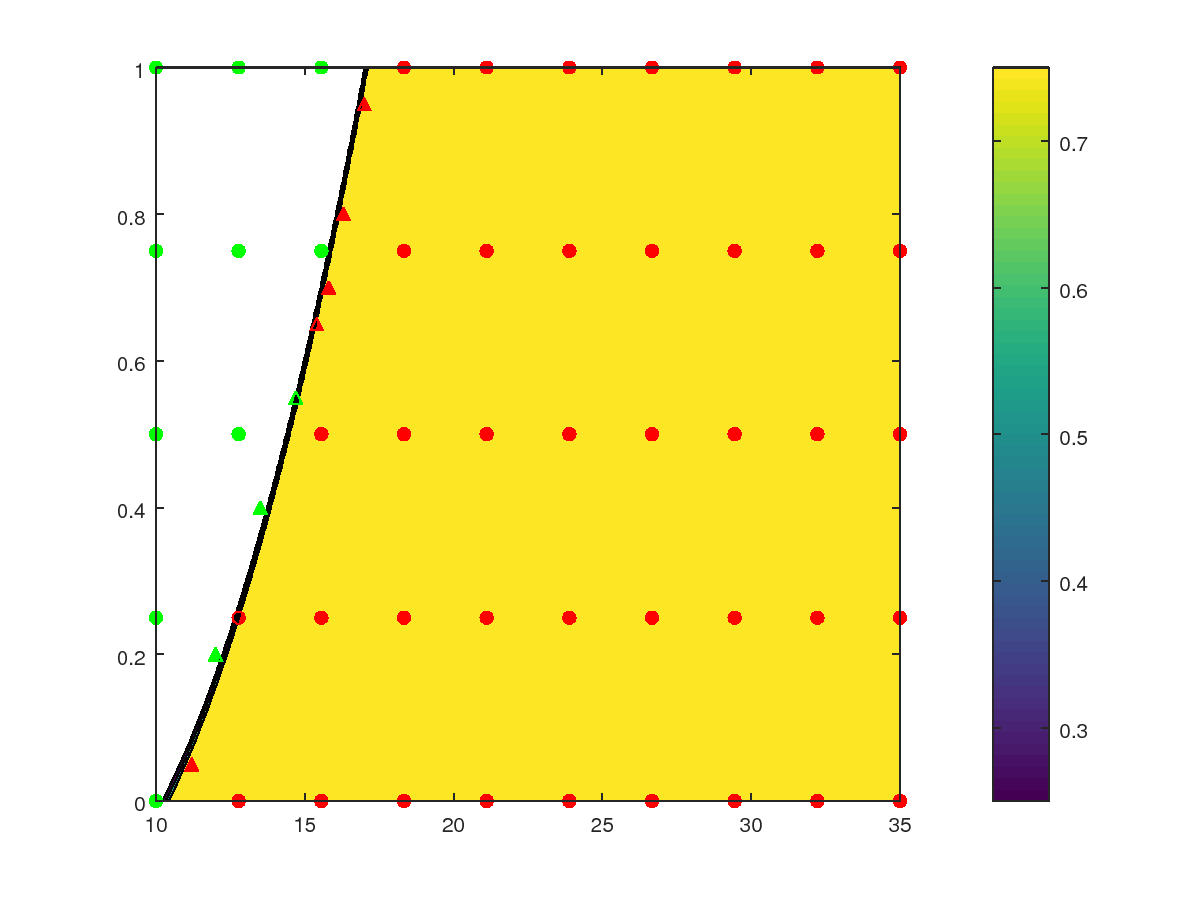
\includegraphics[width=0.75\textwidth]{Figures/classification.png}
  \caption{Binary classification emulator: events reaching $Q_!$ (red) and events not reaching $Q_!$ (green) for $Q_! = XX.X$.}
  \label{fig:classification_Q1}
\end{figure}


\subsubsection{Regression emulator}

\begin{figure}[htpb]
  \centering
  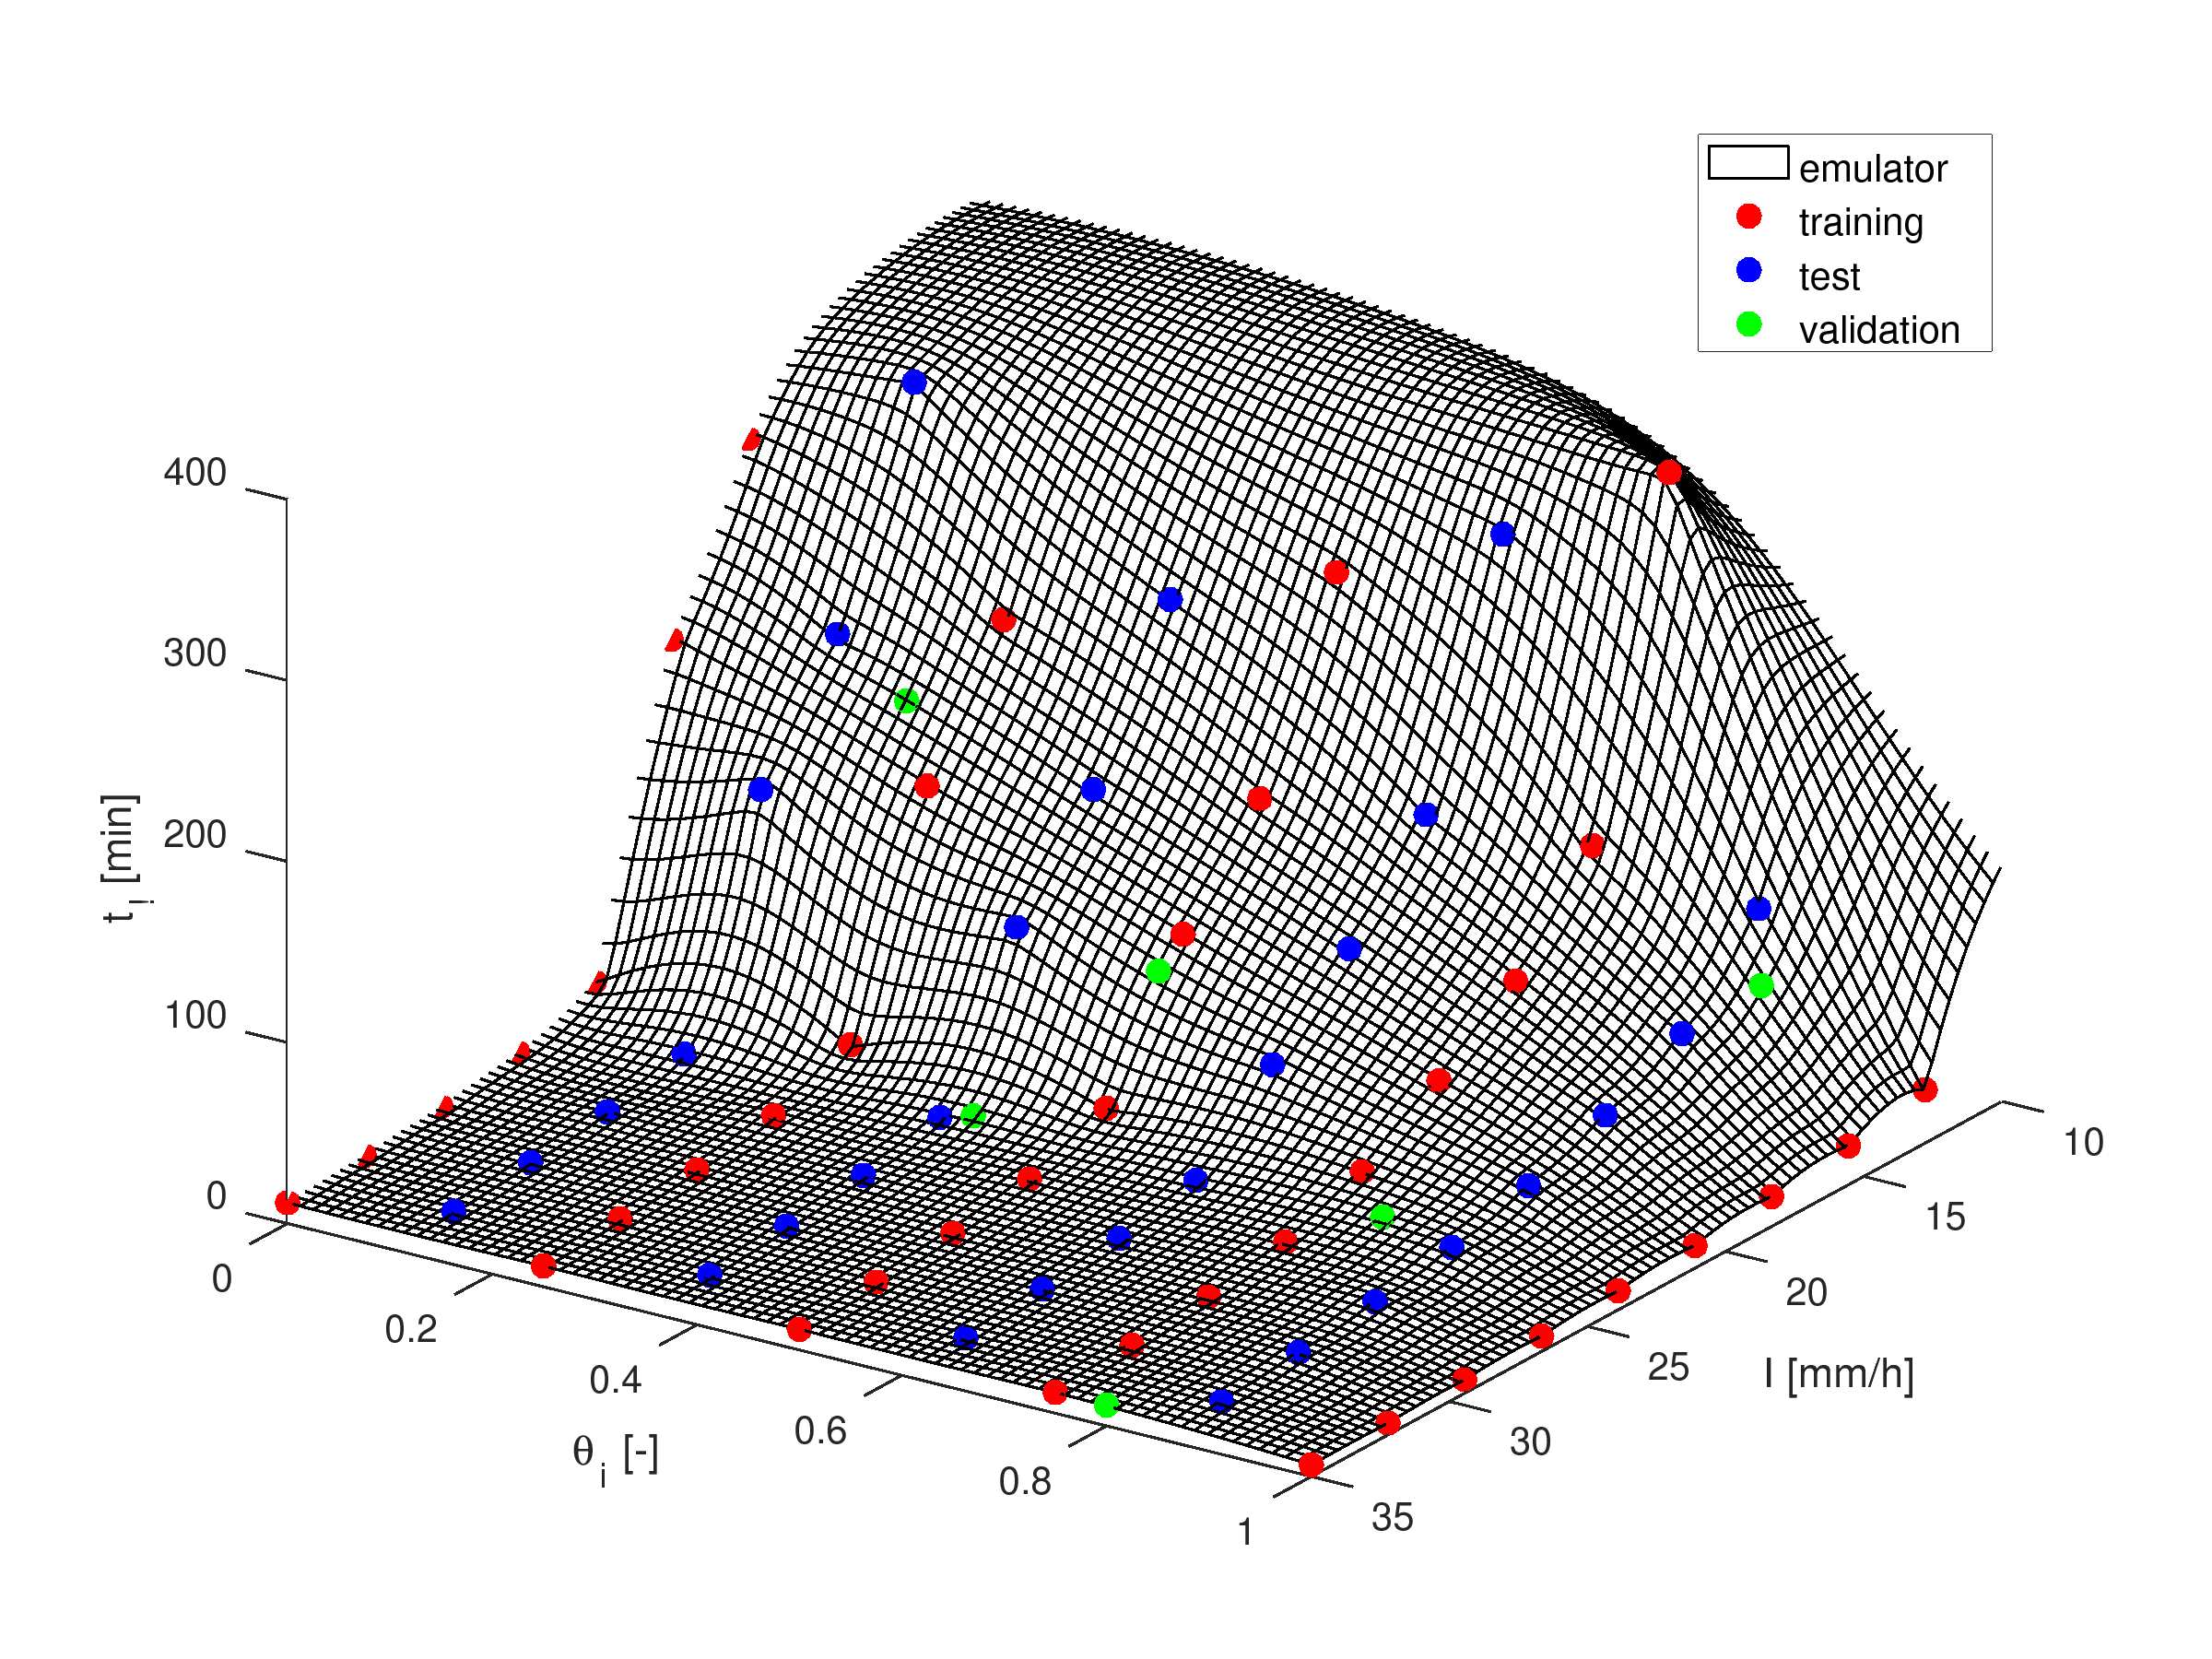
\includegraphics[width=0.7\textwidth]{Figures/emulator.png}
  \caption{Time-to-threshold emulator: training (red), test (blue) and validation (green) datasets and the emulator producing the intrapolation response.}
  \label{fig:regression_emulator}
\end{figure}


\begin{table}[htpb]
  \centering
  \caption{Emulator performance on \emph{test} and \emph{validation} data}
  \label{table label}
  \begin{tabular}{lcc}
    \toprule
     & \textbf{MAE [\si{\minute}, \si{\percent}]} & \textbf{RMSE [\si{\minute}, \si{\percent}]} \\
    \midrule
    \textbf{test} & val & val \\
    \textbf{validation} & val & val \\
    \bottomrule
  \end{tabular}
\end{table}

